\section{Improving Kociemba's Optimal Solver}
Different improvements can be made to our implementation of Kociemba's optimal solver.
	
In the first phase of our implementation of Kociemba's optimal solver it checks if the \cube{} is in \m{H} after every tested move sequence.
This \m{H} is with respect to the primary \face{}s (see subsection \ref{sub:theSubgroupH}). 
It is also possible for the \rubik{} to be inside \m{H} with respect to the secondary or tertiary \face{}s, see figure \ref{fig:secondaryH}.

\begin{figure}[htb]
	\centering
	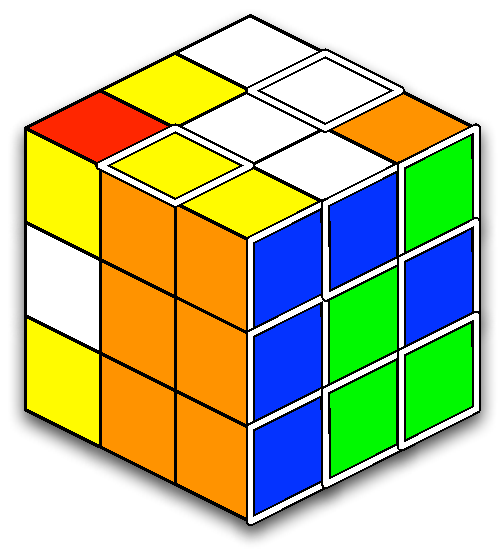
\includegraphics[scale=0.75]{input/pics/secondaryH.pdf}
	\caption{\myCaption{A scrambled Rubik's Cube which is inside secondary \m{H}, but not in primary \m{H}.}}
	\label{fig:secondaryH}
\end{figure}

As with positions in primary \m{H}, the positions in secondary \m{H} must meet the following specifications:
Every secondary \facelet{} must be on the secondary \face{}s, and the edges not in a secondary \face{} must be orientated correctly.
These specifications are met in figure \ref{fig:secondaryH}.

	
When a shortest path to a position is found it could be saved in a lookup table.
If Kociemba's optimal solver gets to a known position it can find the shortests path in the lookup table.
If this is combined with the multiple \m{H} improvement, it could make the search time to get into \m{H} shorter.
 
The program is built up around one \cube{} object.
As a result of this the computer is only able to use one CPU core to work on the \cube{}.
It would be possible to make the application multithreaded in several ways.
With some modifications it could be possible to make a copy of this \cube{} object.
This would make it possible to work on more than one \cube{} object with the same starting position at a time.

When the application is working outside \m{H} it is working with \m{S} moves.
Here it is possible to make a new thread for every depth the method searches in.
In the same way it is possible to make a new thread for every search depth inside \m{H}.

When searching in general the moves in \m{S} and \m{A} could be divided into groups and a new thread could be made for these new groups of moves.